\chapter{Vorstellung des Themas}
\section{Problemdefinition}
Das Aufkommen von Online-Nachrichtenagenturen und die Explosion der Anzahl der Benutzer, die Nachrichten mit diesem Medium konsumieren, haben dazu geführt, dass mehrere Webseiten miteinander konkurrieren, um die Aufmerksamkeit der Benutzer zu erregen. Dies hat dazu geführt, dass Verkaufsstellen kreative Wege geschaffen haben, um Leser auf ihre Website zu locken. Eine der am häufigsten verwendeten Techniken ist die Verwendung von Clickbait-Überschriften. Diese Überschriften wurden speziell entwickelt, um das Interesse des Lesers an dem zu wecken, was versprochen wird, wenn auf den Artikel geklickt wird. Der Artikel liefert normalerweise nicht den Inhalt, den der Leser sucht. 

\section{Lösungsansatz}
Textklassifizierung ist eine gängige Art, wie man \enquote{gute} von \enquote{bösen} Texten unterscheiden kann. Es ist allerdingt nicht praktisch ein großes Sprachmodell wie GPT-3 Browserkompatible zu machen. Erstens ist es völlig \enquote{overkill} für ein solches Problem ein Sprachmodell zu benutzen und zweitens passen diese großen Modelle nicht in den Browser, da die Ladezeit nicht praktisch ist.

Mit dieser Arbeit möchte ich ein Modell erstellen, um Clickbait Überschriften zu erkennen. Es wäre Hilfreich, wenn es ein Dienst gibt, welches eine Überschrift liest und dem Benutzer vorhersagt, ob es sich um Clickbait handelt oder nicht. So kann der Nutzer seine Zeit sparen und muss nicht auf die Seite gehen. Das Hauptprodukt ist dabei dieser Dienst, welches ganz einfach in jede HTML-Seite importiert werden kann. Dieser Dienst muss klein und schnell und gute dabei möglichst Ergebnisse liefern.

\section{Methodik}

Der erste theoretische Teil ist mathematisch/statistsch geprägt. Der zweite theoretische Teil beschäftigt sich mit der Sprache. Es wird nicht scharf zwischen den beiden Kapiteln getrennt, da diese viele Überlappungen haben werden.

Ich werde ein Modell in TensorFlow.js entwickeln. Dieses Modell soll möglichst klein sein und schnell sein. Um mit TensorFlow.js arbeiten zu können muss der Text in Vektoren umgewandelt werden.

Es gibt bereits ein Datensatz \footnote{https://www.kaggle.com/atechnohazard/clickbait-classifier-using-lstm} welches dafür verwendet werden kann. Clickbaits haben ein Muster haben. Das Modell soll dieses Muster erkennen und mit einer relativ hohen Wahrscheinlichkeit sagen, ob es Clickbait ist. Mit einem Versuchsaufbau soll das Modell getestet und analysiert werden. 

Schließlich soll das Modell in die Browser-Umgebung gebracht und mittels eines minimalistischen React Frontends angeboten werden.

\begin{figure}[ht]
  \centering
  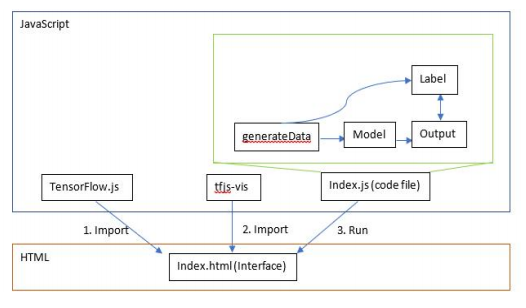
\includegraphics[width=12cm]{kapitel2/beispiel.png}
  \caption[Beispiel einer Systemarchitektur]{Beispiel einer Systemarchitektur entnommen aus \cite{cho2019shop}. Der Client bekommt beim laden der Seite, neben dem HTML, CSS und dem JavaScript, welches für das Frontend nötig ist, ein weiteres Script, welches die TensorFlow.js API bereitstellt. Die Berechnung findet im Browser, beim Client statt, wo auch das Modell sich befindet.}
  \label{Kap2:SystemArchitektur}
\end{figure}
 
\section{Wissenschaftlicher Beitrag}
\begin{itemize}
  \item Den Stand der Technik in Bezug auf Deep Learning und Worteinbettungen zeigen
  \item Implementierung eines NLP-Problemes im Browser ohne zusätzliche Software oder Plugins, mit TensorFlow.js
  \item Optimierung des Browsers für Deep Learning 
  \item Auswahl des optimalen Modells und der Trainingsmethode
  \item Produktion eines Dienstes, um Clickbait Nachrichten vorzubeugen
\end{itemize}

\section{Einstiegsliteratur}

\begin{itemize}
  \item \cite{kaur2020detecting}
  \item \cite{Chavan2019}
  \item \cite{vorakitphan2018clickbait}
  \item \cite{anand2017we}
  \item \cite{gairola2017neural}
  \item \cite{kumar2018identifying}
  \item \cite{glenski2017fishing}
  \item \cite{chawda2019novel}
  \item \cite{seopredicting}
  \item \cite{cho2019shop}
  \item \cite{roberts2018magenta}
  \item \cite{aggarwal2012survey}
  \item \cite{kowsari2019text}
  \item \cite{korde2012text}
  \item \cite{altinel2018semantic}
  \item \cite{nordberg2020crucial}
  \item \cite{raamkumar2020use}
  \item \cite{rivera2020identifying}
  \item \cite{nguyen2020real}
  \item \cite{zhang2015character}
  \item \cite{kiranyaz20191d}
  \item \cite{severyn2015unitn}
  \item \cite{severyn2015twitter}
  \item \cite{zhao2019speech}
  \item \cite{eren2019generic}
\end{itemize}

\section{Grobgliederung}
\renewcommand{\labelenumii}{\theenumii}
\renewcommand{\theenumii}{\theenumi.\arabic{enumii}.}

\begin{enumerate}

  \item Einleitung
  \begin{enumerate}
    \item Motivation
    \item Wissenschaftlicher Beitrag
    \item Struktur der Arbeit
  \end{enumerate}

  \item Neuronale Netze
  \begin{enumerate}
    \item Einleitung
    \item Arten des Neuronalen Lernens
    \item Netzwerkparameter und Hyperparameter
    \item Aktivierungsfunktionen
    \item Verlustfunktion
    \item Optimizer
    \item Epochen
    \item TensorFlow.js
    \item Schluss
  \end{enumerate}

  \item Die natürliche Sprache
  \begin{enumerate}
    \item Einleitung
    \item Vektorisierung des Textes durch Encoding
    \item Worteinbettungen
    \item 1d CNN
    \item Schluss
  \end{enumerate}

  \item Aktueller Forschungsstand
  \begin{enumerate}
  \item Einleitung
  \item Clickbaits und Deep Learning Ansätze
  \item TensorFlow.js 
  \item Worteinbettungen
  \end{enumerate}

  \item Methodik
  \begin{enumerate}
    \item Einleitung
    \item Die Systemarchitektur
    \item JavaScript
    \item Explorative Datenanalyse
    \item Datenverarbeitung und Feature Engineering
    \item Modelling
    \item Das Zusammenbringen des Modells mit dem Frontend
    \item Schluss
  \end{enumerate}

  \item Versuchsaufbau und Diskussion der Ergebnisse
  \begin{enumerate}
    \item Einleitung
    \item Anpassung der Netzwerkparameter und Hyperparameter
    \item Leistungsmessungen
    \item Vergleich und Darstellung der Ergebnisse
    \item Schluss
  \end{enumerate}

  \item Schluss
  \begin{enumerate}
    \item Fazit zum Forschungsbeitrag
    \item Abschließende Gedanken
    \item Zukunft der Arbeit
  \end{enumerate}
\end{enumerate}




% \section{Hervorhebungen}
% \label{Einleitung:Textauszeichnungen}

% Achten Sie bitte auf die grundlegenden Regeln der Typographie\index{Typographie}\footnote{Ein Ratgeber in allen Detailfragen ist \cite{Forssman2002}.}, wenn Sie Ihren Text schreiben. Hierzu gehören z.\,B. die Verwendung der richtigen "`Anführungszeichen"' und der Unterschied zwischen Binde- (-), Gedankenstrich (--) und langem Strich (---). Sie erhalten den Bindestrich in \LaTeX{} mit \verb+-+, den Gedankenstrich mit \verb+--+ und den langen Strich mit \verb+---+.

% Wenn Sie Text hervorheben wollen, dann setzten Sie ihn mit \verb+\textit+ \textit{kursiv} (Italic) und nicht \textbf{fett} (Bold). Fettdruck ist Überschriften vorbehalten; im Fließtext stört er den Lesefluss. Das \underline{Unterstreichen} von Fließtext ist im gesamten Dokument tabu und kann maximal bei Pseudo"=Code vorkommen.\index{Hervorhebungen}


% \section{Anführungszeichen}

% Deutsche Anführungszeichen werden mit \verb+"`+ und \verb+"'+ erzeugt: "`dieser Text steht in \glq Anführungszeichen\grq; alles klar?"'. Englische Anführungszeichen hingegen mit \verb+``+ und \verb+''+: ``this is an `English' quotation''. Beachten Sie, dass Sie in Zitaten immer die zur Sprache passenden Anführungszeichen verwenden. Die Verwendung von \verb+"+ ist für Anführungszeichen immer falsch und führt bei \LaTeX{} zu seltsamen "Effekten".

% Um sich diesen Ärger zu sparen, biete sich die Verwendung des Paketes \textit{csquotes} und des Kommandos \verb+\enquote+ an. Hierdurch werden die Anführungszeichen korrekt für die eingestellte Sprache gesetzt und Sie müssen sich \enquote{keine Sorgen mehr über die \enquote{Anführungszeichen} machen}.


% \section{Abkürzungen}
% \index{Abkürzungen}
% \index{Abbreviation|see{Abkürzungen}}

% Eine \ac{ABK} (\verb+\ac{ABK}+) wird bei der ersten Verwendung ausgeschrieben. Danach nicht mehr: \ac{ABK}. Man kann allerdings mit \verb+\acl+ die Langform explizit anfordern (\acl{ABK}) oder mit \verb+\acs+ die Kurzform (\acs{ABK}) oder mit \verb+\acf+ auch noch einmal die Definition (\acf{ABK}).

% Beachten Sie, dass bei Abkürzungen, die für zwei Wörter stehen, ein kleines Leerzeichen nach dem Punkt kommt: z.\,B. bzw. \zb{} und d.\,h. bzw. \dahe{}. Das Template bietet hierfür die beiden Makros \verb+\zb{}+ und \verb+\dahe{}+.


% \section{Querverweise}

% Querverweise auf eine Kapitelnummer macht man im Text mit \verb+\ref+ (Kapitel~\ref{Einleitung:Textauszeichnungen}) und auf eine bestimmte Seite mit \verb+\pageref+ (Seite~\pageref{Einleitung:Textauszeichnungen}). Man kann auch den Befehl \verb+\autoref+ benutzen, der automatisch die Art des referenzierten Elements bestimmt (\zb{} \autoref{Einleitung:Textauszeichnungen} oder \autoref{Kap2:Kopplungsformen}).


% \section{Fußnoten}

% Fußnoten werden einfach mit in den Text geschrieben und zwar genau an die Stelle\footnote{An der die Fußnote auftauchen soll}. Hierzu dient der Befehl \verb+\footnote{Text}+.


% \section{Tabellen}

% Tabellen werden normalerweise ohne vertikale Striche gesetzt, sondern die Spalten werden durch einen entsprechenden Abstand voneinander getrennt.\footnote{Siehe \cite[S. 89]{Willberg1999}.} Zum Einsatz kommen ausschließlich horizontale Linien (siehe Tabelle~\ref{Kap2:Kopplungsformen}).

% \begin{table}[h]
%   \caption{Ebenen der Kopplung und Beispiele für enge und lose Kopplung}
%   \label{Kap2:Kopplungsformen}
%   \renewcommand{\arraystretch}{1.2}
%   \centering
%   \sffamily
%   \begin{footnotesize}
%     \begin{tabular}{l l l}
%     \toprule
%     \textbf{Form der Kopplung} & \textbf{enge Kopplung} & \textbf{lose Kopplung}\\
%     \midrule
%     Physikalische Verbindung	&	Punkt-zu-Punkt	& 	über Vermittler\\
%     Kommunikationsstil	&	synchron		&	asynchron\\
%     Datenmodell	&	komplexe gemeinsame Typen	&	nur einfache gemeinsame Typen\\
%     Bindung	&	statisch		&	dynamisch\\
%     \bottomrule
%     \end{tabular}
%   \end{footnotesize}
%   \rmfamily
% \end{table}

% Eine Tabelle fließt genauso, wie auch Bilder durch den Text. Siehe Tabelle~\ref{Kap2:Kopplungsformen}.

% Manchmal möchte man Tabellen, in denen der Text in der Tabellenspalte umbricht. Hierzu dient die Umgebung \texttt{tabularx}, wobei \texttt{L} eine Spalte mit Flattersatz und \texttt{X} eine mit Blocksatz definiert. Die Breite der Tabelle kann über den Faktor vor \verb+\textwidth+ angegeben werden.

% \begin{table}[h]
%   \caption{Teildisziplinen der Informatik}
%   \label{Kap2:Teildisziplinen}
%   \renewcommand{\arraystretch}{1.2}
%   \centering
%   \sffamily
%   \begin{footnotesize}
%     \begin{tabularx}{0.9\textwidth}{l X L}
%       \toprule
%       \textbf{Gebiet} & \textbf{Definition} & \textbf{Beispiel}\\
%       \midrule
%       \emph{Praktische Informatik} & Informatik-Disziplinen, welche sich vorwiegend mit der Entwicklung und Anwendung der Software-Komponenten befassen & Programmentwicklung, Compilerbau; im Aufbau von z.B. Informationssystemen und Netzwerken ergeben sich Überlappungen mit der technischen Informatik \\
%       \emph{Technische Informatik} & Informatik-Disziplinen, welche sich vorwiegend mit der Entwicklung und Anwendung der Hardware-Komponenten befassen & Digitaltechnik, Mikroprozessortechnik \\
%       \emph{Theoretische Informatik} & Informatik-Disziplinen, welche sich mit der Entwicklung von Theorien und Modellen der Informatik befassen und dabei viel Substanz aus der Mathematik konsumieren & Relationenmodell, Objekt-Paradigmen, Komplexitätstheorie, Kalküle \\
%       \emph{Angewandte Informatik} & Informatik als instrumentale Wissenschaft & Rechtsinformatik, Wirtschaftsinformatik, Geoinformatik \\
%       \bottomrule
%     \end{tabularx}
%   \end{footnotesize}
%   \rmfamily
% \end{table}


% \section{Harveyballs}

% \begin{quote}
%     Harvey Balls sind kreisförmige Ideogramme, die dazu dienen, qualitative Daten anschaulich zu machen. Sie werden in Vergleichstabellen verwendet, um anzuzeigen, inwieweit ein Untersuchungsobjekt sich mit definierten Vergleichskriterien deckt. \parencite{Wikipedia_HarveyBalls}
% \end{quote}

% \begin{table}[h]
%   \caption{Beispiel für Harvey Balls}
%   \label{tab:harveyexample}
%   \centering
%   \begin{tabular}{lccc}
%     \toprule
%     & Ansatz 1 & Ansatz 2 & Ansatz 3\\
%     \midrule
%     Eigenschaft 1	& \harveyBallNone & \harveyBallQuarter & \harveyBallHalf \\
%     Eigenschaft 2	& \harveyBallHalf & \harveyBallThreeQuarter & \harveyBallFull \\
%     Eigenschaft 3	& \harveyBallFull & \harveyBallThreeQuarter & \harveyBallQuarter\\
%     \bottomrule
%   \end{tabular}
% \end{table}


% \section{Aufzählungen}

% Aufzählungen sind toll.

% \begin{itemize}
%   \item Ein wichtiger Punkt
%   \item Noch ein wichtiger Punkt
%   \item Ein Punkt mit Unterpunkten
%     \begin{itemize}
%       \item Unterpunkt 1
%       \item Unterpunkt 2
%     \end{itemize}
%   \item Ein abschließender Punkt ohne Unterpunkte
% \end{itemize}


% Aufzählungen mit laufenden Nummern sind auch toll.

% \begin{enumerate}
%   \item Ein wichtiger Punkt
%   \item Noch ein wichtiger Punkt
%   \item Ein Punkt mit Unterpunkten
%     \begin{enumerate}
%       \item Unterpunkt 1
%       \item Unterpunkt 2
%     \end{enumerate}
%   \item Ein abschließender Punkt ohne Unterpunkte
% \end{enumerate}
